% Michael Linder  <mplinder@utexas.edu>
% Master's Report document 
%
% Major: Computer and Electrical Engineering
% Focus: Software Engineering
% Cockrell School of Engineering
% The University of Texas at Austin
%
% Based on the UT LaTeX package provided at:
% http://www.utexas.edu/ogs/etd/LaTeX/


\documentclass[12pt]{report}	% The documentclass must be ``report''.

\usepackage{utdiss2}  		% Dissertation package style file.


%%%%%%%%%%%%%%%%%%%%%%%%%%%%%%%%%%%%%%%%%%%%%%%%%%%%%%%%%%%%%%%%%%%%%%
% Optional packages used for this sample dissertation. If you don't  %
% need a capability in your dissertation, feel free to comment out   %
% the package usage command.					     %
%%%%%%%%%%%%%%%%%%%%%%%%%%%%%%%%%%%%%%%%%%%%%%%%%%%%%%%%%%%%%%%%%%%%%%

\usepackage{amsmath,amsthm,amsfonts,amscd} 
				% Some packages to write mathematics.
\usepackage{eucal} 	 	     % Euler fonts
\usepackage{verbatim}      % Allows quoting source with commands.
\usepackage{makeidx}       % Package to make an index.
\usepackage{graphicx}         	% Allows inclusion of eps files.
\usepackage{citesort}         % 
\usepackage{url}		% Allows good typesetting of web URLs.
\usepackage{draftwatermark}		% Uncomment this line to have the
				% word, "DRAFT," as a background
				% "watermark" on all of the pages of
				% of your draft versions. When ready
				% to generate your final copy, re-comment
				% it out with a percent sign to remove
				% the word draft before you re-run
				% Makediss for the last time.
\SetWatermarkScale{4}

\author{Michael Linder}  	% Required

\address{mplinder@utexas.edu}  % Required

\title{Honeycomb: Indoor location estimation based on Wi-Fi signal strength}
                                                    % Required

%%%%%%%%%%%%%%%%%%%%%%%%%%%%%%%%%%%%%%%%%%%%%%%%%%%%%%%%%%%%%%%%%%%%%%
% NOTICE: The total number of supervisors and other members %%%%%%%%%%
%%%%%%%%%%%%%%% MUST be seven (7) or less! If you put in more, %%%%%%%
%%%%%%%%%%%%%%% they are put on the page after the Committee %%%%%%%%%
%%%%%%%%%%%%%%% Certification of Approved Version page. %%%%%%%%%%%%%%
%%%%%%%%%%%%%%%%%%%%%%%%%%%%%%%%%%%%%%%%%%%%%%%%%%%%%%%%%%%%%%%%%%%%%%

%%%%%%%%%%%%%%%%%%%%%%%%%%%%%%%%%%%%%%%%%%%%%%%%%%%%%%%%%%%%%%%%%%%%%%
%
% Enter names of the supervisor and co-supervisor(s), if any,
% of your dissertation committee. Put one name per line with
% the name in square brackets. The name on the last line, however,
% must be in curly braces.
%
% If you have only one supervisor, the entry below will read:
%
%	\supervisor
%		{Supervisor's Name}
%
% NOTE: Maximum three supervisors. Minimum one supervisor.
% NOTE: The Office of Graduate Studies will accept only two supervisors!
% 
%
\supervisor
	{Christine Julien}

%%%%%%%%%%%%%%%%%%%%%%%%%%%%%%%%%%%%%%%%%%%%%%%%%%%%%%%%%%%%%%%%%%%%%%
%
% Enter names of the other (non-supervisor) members(s) of your
% dissertation committee. Put one name per line with the name
% in square brackets. The name on the last line, however, must
% be in curly braces.
%
% NOTE: Maximum six other members. Minimum zero other members.
% NOTE: The Office of Graduate Studies may restrict you to a total
%	of six committee members.
%
%
\committeemembers
	{William Bard}

%%%%%%%%%%%%%%%%%%%%%%%%%%%%%%%%%%%%%%%%%%%%%%%%%%%%%%%%%%%%%%%%%%%%%%

\previousdegrees{B.A.}
     % The abbreviated form of your previous degree(s).
     % E.g., \previousdegrees{B.S., MBA}.
     %
     % The default value is `B.S., M.S.'

\graduationmonth{May}      
     % Graduation month, either May, August, or December, in the form
     % as `\graduationmonth{May}'. Do not abbreviate.
     %
     % The default value (either May, August, or December) is guessed
     % according to the time of running LaTeX.

\graduationyear{2015}   
     % Graduation year, in the form as `\graduationyear{2001}'.
     % Use a 4 digit (not a 2 digit) number.
     %
     % The default value is guessed according to the time of 
     % running LaTeX.

%\typist{...}       
     % The name(s) of typist(s), put `the author' if you do it yourself.
     % E.g., `\typist{Maryann Hersey and the author}'.
     %
     % The default value is `the author'.


%%%%%%%%%%%%%%%%%%%%%%%%%%%%%%%%%%%%%%%%%%%%%%%%%%%%%%%%%%%%%%%%%%%%%%
% Commands for master's theses and reports.			     %
%%%%%%%%%%%%%%%%%%%%%%%%%%%%%%%%%%%%%%%%%%%%%%%%%%%%%%%%%%%%%%%%%%%%%%
%
% If the degree you're seeking is NOT Doctor of Philosophy, uncomment
% (remove the % in front of) the following two command lines (the ones
% that have the \ as their second character).
%
\degree{Master of Science in Engineering}
\degreeabbr{M.S.E.}

% Uncomment the line below that corresponds to the type of master's
% document you are writing.
%
\masterreport
%\masterthesis


%%%%%%%%%%%%%%%%%%%%%%%%%%%%%%%%%%%%%%%%%%%%%%%%%%%%%%%%%%%%%%%%%%%%%%
% Some optional commands to change the document's defaults.	     %
%%%%%%%%%%%%%%%%%%%%%%%%%%%%%%%%%%%%%%%%%%%%%%%%%%%%%%%%%%%%%%%%%%%%%%
%
%\singlespacing
%\oneandonehalfspacing

%\singlespacequote
\oneandonehalfspacequote

\topmargin 0.125in	% Adjust this value if the PostScript file output
			% of your dissertation has incorrect top and 
			% bottom margins. Print a copy of at least one
			% full page of your dissertation (not the first
			% page of a chapter) and measure the top and
			% bottom margins with a ruler. You must have
			% a top margin of 1.5" and a bottom margin of
			% at least 1.25". The page numbers must be at
			% least 1.00" from the bottom of the page.
			% If the margins are not correct, adjust this
			% value accordingly and re-compile and print again.
			%
			% The default value is 0.125"

		% If you want to adjust other margins, they are in the
		% utdiss2-nn.sty file near the top. If you are using
		% the shell script Makediss on a Unix/Linux system, make
		% your changes in the utdiss2-nn.sty file instead of
		% utdiss2.sty because Makediss will overwrite any changes
		% made to utdiss2.sty.

%%%%%%%%%%%%%%%%%%%%%%%%%%%%%%%%%%%%%%%%%%%%%%%%%%%%%%%%%%%%%%%%%%%%%%
% Some optional commands to be tested.				     %
%%%%%%%%%%%%%%%%%%%%%%%%%%%%%%%%%%%%%%%%%%%%%%%%%%%%%%%%%%%%%%%%%%%%%%

% If there are 10 or more sections, 10 or more subsections for a section,
% etc., you need to make an adjustment to the Table of Contents with the
% command \longtocentry.
%
%\longtocentry 



%%%%%%%%%%%%%%%%%%%%%%%%%%%%%%%%%%%%%%%%%%%%%%%%%%%%%%%%%%%%%%%%%%%%%%
%	Some math support.					     %
%%%%%%%%%%%%%%%%%%%%%%%%%%%%%%%%%%%%%%%%%%%%%%%%%%%%%%%%%%%%%%%%%%%%%%
%
%	Theorem environments (these need the amsthm package)
%
%% \theoremstyle{plain} %% This is the default

\newtheorem{thm}{Theorem}[section]
\newtheorem{cor}[thm]{Corollary}
\newtheorem{lem}[thm]{Lemma}
\newtheorem{prop}[thm]{Proposition}
\newtheorem{ax}{Axiom}

\theoremstyle{definition}
\newtheorem{defn}{Definition}[section]

\theoremstyle{remark}
\newtheorem{rem}{Remark}[section]
\newtheorem*{notation}{Notation}

%\numberwithin{equation}{section}


%%%%%%%%%%%%%%%%%%%%%%%%%%%%%%%%%%%%%%%%%%%%%%%%%%%%%%%%%%%%%%%%%%%%%%
%	Macros.							     %
%%%%%%%%%%%%%%%%%%%%%%%%%%%%%%%%%%%%%%%%%%%%%%%%%%%%%%%%%%%%%%%%%%%%%%
%
%	Here some macros that are needed in this document:


\newcommand{\latexe}{{\LaTeX\kern.125em2%
                      \lower.5ex\hbox{$\varepsilon$}}}

\newcommand{\amslatex}{\AmS-\LaTeX{}}

\chardef\bslash=`\\	% \bslash makes a backslash (in tt fonts)
			%	p. 424, TeXbook

\newcommand{\cn}[1]{\texttt{\bslash #1}}

\makeatletter		% Starts section where @ is considered a letter
			% and thus may be used in commands.
\def\square{\RIfM@\bgroup\else$\bgroup\aftergroup$\fi
  \vcenter{\hrule\hbox{\vrule\@height.6em\kern.6em\vrule}%
                                              \hrule}\egroup}
\makeatother		% Ends sections where @ is considered a letter.
			% Now @ cannot be used in commands.

\makeindex    % Make the index

%%%%%%%%%%%%%%%%%%%%%%%%%%%%%%%%%%%%%%%%%%%%%%%%%%%%%%%%%%%%%%%%%%%%%%
%		The document starts here.			     %
%%%%%%%%%%%%%%%%%%%%%%%%%%%%%%%%%%%%%%%%%%%%%%%%%%%%%%%%%%%%%%%%%%%%%%

\begin{document}

\copyrightpage          % Produces the copyright page.


%
% NOTE: In a doctoral dissertation, the Committee Certification page
%		(with signatures) is BEFORE the Title page.
%	In a masters thesis or report, the Signature page
%		(with signatures) is AFTER the Title page.
%
%	If you are writing a masters thesis or report, you MUST REVERSE
%	the order of the \commcertpage and \titlepage commands below.
%

\titlepage              % Produces the title page.

\commcertpage           % Produces the Committee Certification
			%   of Approved Version page (doctoral)
			%   or Signature page (masters).
			%		20 Mar 2002	cwm



%%%%%%%%%%%%%%%%%%%%%%%%%%%%%%%%%%%%%%%%%%%%%%%%%%%%%%%%%%%%%%%%%%%%%%
% Dedication and/or epigraph are optional, but must occur here.      %
%%%%%%%%%%%%%%%%%%%%%%%%%%%%%%%%%%%%%%%%%%%%%%%%%%%%%%%%%%%%%%%%%%%%%%
%
\begin{dedication}
\index{Dedication@\emph{Dedication}}%
Dedicated to my wife, Dana, whose support made this possible.
\end{dedication}


% \begin{acknowledgments}		% Optional
% \index{Acknowledgments@\emph{Acknowledgments}}%
% TODO: ACKNOWLEDGMENTS \ldots
% \end{acknowledgments}


% The abstract is required. Note the use of ``utabstract'' instead of
% ``abstract''! This was necessary to fix a page numbering problem.
% The abstract heading is generated automatically.
% Do NOT use \begin{abstract} ... \end{abstract}.
%
\utabstract
\index{Abstract}%
\indent

TODO: fix this. it's awful
This paper presents Honeycomb, an indoor location estimation product based on Wi-Fi signal strength. Wireless Local Area Networks are ubiquitous today, and most people carry Wi-Fi capable devices in their pocket.  This existing infrastructure can thus be leveraged for purposes of location estimation. Using Wi-Fi signal strength fingerprinting, Honeycomb harnesses existing Wi-Fi infrastructures as a means to track the movements of individuals through a space. Fingerprinting is a method by which Wi-Fi signal strengths are mapped at regular intervals in a bounded space. Once a space is fingerprinted, a given node must simply sample Wi-Fi signal strengths as it moves through the same space and Honeycomb's algorithm will determine the node's path in an offline manner.


\tableofcontents   % Table of Contents will be automatically
                   % generated and placed here.

\listoftables      % List of Tables and List of Figures will be placed
\listoffigures     % here, if applicable.



%%%%%%%%%%%%%%%%%%%%%%%%%%%%%%%%%%%%%%%%%%%%%%%%%%%%%%%%%%%%%%%%%%%%%%
% Actual text starts here.					     %
%%%%%%%%%%%%%%%%%%%%%%%%%%%%%%%%%%%%%%%%%%%%%%%%%%%%%%%%%%%%%%%%%%%%%%
%
% Including external files for each chapter makes this document simpler,
% makes each chapter simpler, and allows for generating test documents
% with as few as zero chapters (by commenting out the include statements).
% This allows quicker processing by the Makediss command file in case you
% are not working on a specific, long and slow to compile chapter. You
% can even change the chapter order by merely interchanging the order
% of the include statements (something I found helpful in my own
% dissertation).
%
\chapter{Introduction}
\label{introduction}
\index{Introduction@\emph{Introduction}}%


In recent years wireless LAN technology has become ubiquitous. Wi-Fi access points have become virtually trivial to install, and nearly everyone carries a Wi-Fi capable mobile device in their pocket. It is also the case that much research has been done on various methods of location estimation. It follows, then, that location estimation that leverages Wi-Fi would be a valuable topic, and in fact much research has already been done in the space, including \cite{ito2005bayesian}, \cite{liu2007survey}, \cite{kawaguchi2009wifi}, \cite{hotta2012robust}, and \cite{nagaosa2012dept}. 

The benefits of using Wi-Fi for location estimation are manifold. For instance, while the Global Positioning System is in many ways the premier method for location estimation in the world \cite{bajaj2002gps}, GPS signals are often unreliable indoors \cite{xiong2012towards}, making it a poor choice for any indoor location estimation. Location systems that use other mechanisms such as RFID \cite{toplan2012rfid}, radio waves, ultrasound \cite{priyantha2005cricket}, or geomagnetism \cite{chung2011indoor} are difficult to setup, require specialized hardware, and ultimately can only be used for a single purpose. Wi-Fi based location estimation solves all of these problems. Wi-Fi signals are readily available indoors. Wi-Fi is relatively cheap and easy to setup, and in many cases existing access points can be leveraged.

\section{Definitions}
\index{Definitions@\emph{Definitions}}%

There are a few terms that will be used throughout this paper that it is important to define early. Understanding these definitions will help make clear the purpose of this paper and its contributions. 

\paragraph{Signal Strength vs. RSSI}

Much of the research involving location estimation with Wi-Fi signal strength refers to the measured power present in the radio signal as the Received Signal Strength Indicator (RSSI). While in general terms this moniker is good enough, in truth, the IEEE 802.11 specifications \cite{ieee802.11} do not indicate a specific relationship between RSSI and the actual power level as measured in either milliwatts (mW) or Decibel-milliwatts (dBm). As such manufactures are free to provide their own arbitrary units, and RSSI measurements are generally found to be integer values greater than 0. Because of this inconsistency, Honeycomb does not use RSSI, favoring instead what we refer to as simply "signal strength". For our purposes, signal strength is a measure of the power present in the Wi-Fi signal as measured in dBm. dBm is a measurement relative to 1 mW of power, where 0 dBm is equal to 1 mW. Because dBm measurements are made on a logarithmic scale, we find our measurements to be negative integers between 0 and 100, where the measured value is the exponent in the logarithm. So, where 0 dBm is equal to 1 mW, -10 dBm is equal to .1 mW, -20 dBm is equal to .01 mW, and so on. Measuring signal strength in this way allows Honeycomb to maintain consistent tracking across signal strength measurement platforms, and thus makes Honeycomb a more diverse and viable product.


\paragraph{Fingerprint}
Throughout this paper will we refer to fingerprints. In this context, a fingerprint is a set of Wi-Fi signal strength measurements taken from a set of Wi-Fi access points at a specific point in a given space. 

\begin{figure}[htb] % Imported eps example.
	\begin{center}
		\ 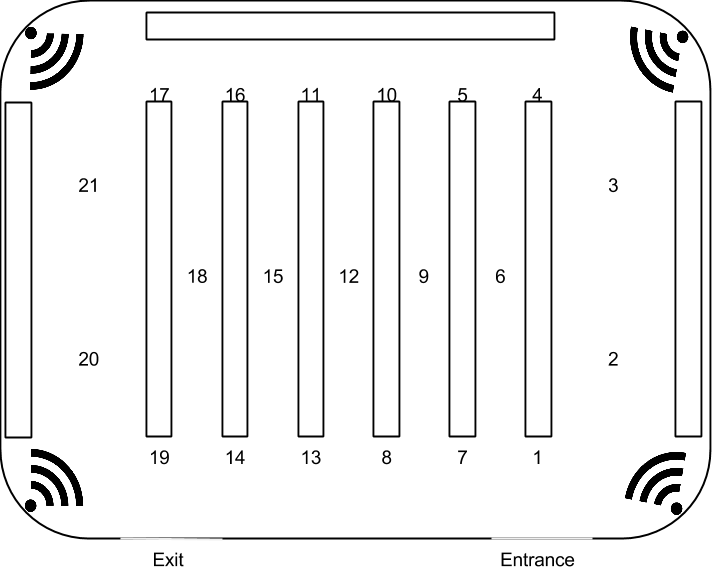
\includegraphics[width=4in,height=3in]{ExampleLocation.png}
		\caption{An example of a location with labeled measurement points}
		\label{storeexample}
	\end{center}
\end{figure}


\paragraph{Fingerprint Session}

While the concept of the Wi-Fi fingerprint is relatively common, here we introduce a new concept that will enable a Honeycomb installation to maintain its value over time: the fingerprint session. A fingerprint session is the complete set of fingerprints from all points in a space at any given time. Because the internal layout of any given space can change over time, causing issues with blocking and reflection of Wi-Fi signals, Honeycomb has built in the ability to re-fingerprint the entire location at any time so that the measurements can be as precise as possible. Figure \ref{storeexample} shows an example location with aisles like that of a grocery store. It includes four Wi-Fi access points and numbered labels for points that may be considered relevant for location estimation. A single fingerprint session in this space would be the complete set of Wi-Fi signal strength measurements from all four access points at every numbered location. 


\paragraph{User Track}
A user track differs from a fingerprint in that it represents a single user's movement through the space. Thus, a user track is composed of a set of timestamps, each of which is associated with a set of signal strength measurements for each of the access points in the space. Figure \ref{usertrackexample} shows an example of a user track. In this example, the small dots represent the user's actual path through the space, while each large dot represents a timestamped set of signal strength measurements. Thus it can be seen that in this example that the user walked at a relatively constant pace through the space, slowing down four times near locations 5, 7, 14, and 17. For location estimation purposes, Honeycomb will compare a given user track to the most recent fingerprint session for the given space. 


\begin{figure}[htb] % Imported eps example.
	\begin{center}
		\ 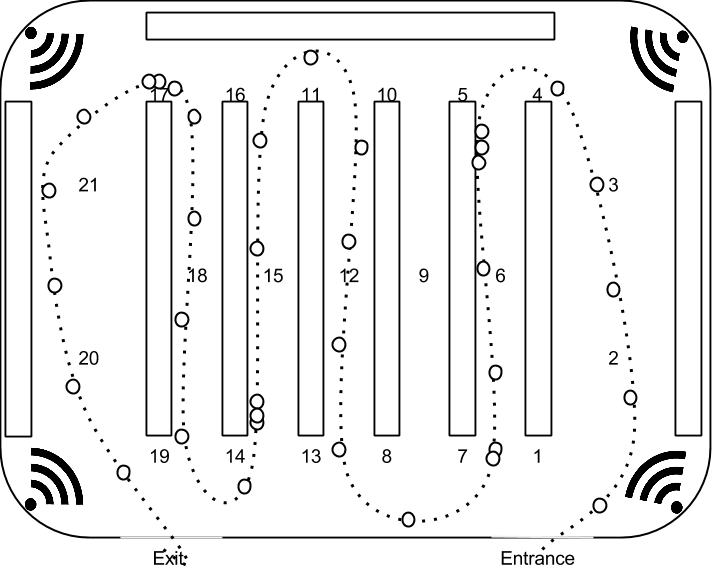
\includegraphics[width=4in,height=3in]{ExampleUserTrack.png}
		\caption{An example user track}
		\label{usertrackexample}
	\end{center}
\end{figure}


\section{Motivation}
\index{Motivation@\emph{Motivation}}%

Wi-Fi based location estimation is a well researched topic \cite{liu2007survey}. The goal of Honeycomb is to leverage that research and build an indoor location tracking system which is suitable for deployment in a real world scenario.  As such, Honeycomb includes an Android application capable of fingerprinting a space, and an API which is deployed to the web for uploading both fingerprints and user track data. The web application also executes the location estimation algorithm, and provides a user interface for browsing the user track data. Honeycomb itself remains agnostic of the mechanism used to gather the user's Wi-Fi signal strength data. By decoupling Honeycomb in this way, we allow Honeycomb to be used in multiple scenarios in which a specialized user track gathering mechanism is desired. 

User privacy is also a major motivating factor in our work. By only performing location estimation based on signal strength and timestamp data passively gathered on the Wi-Fi capable device, we have avoided the pitfalls of systems that require the mobile device to send out a beacon \cite{ito2005bayesian} \cite{xiong2012towards} which can be intercepted by malicious third parties. Additionally, the offline nature of the location estimation algorithm greatly simplifies the entire process, as real time location estimation is still a highly volatile field \cite{turner2011empirical}. It also helps provide an additional layer of privacy protection for the user, as the data can easily be decoupled from any identifying information before processing.
 
 
\section{Contribution}
\index{Contribution@\emph{Contribution}}%

While there has been much research done in the space, to the author's knowledge, there does not yet exist a product on the market that achieves true location estimation via Wi-Fi signal strength measurements. Honeycomb is such a product. Honeycomb provides tools on the web for site administrators to manage their locations and view individual user tracks. It also includes an API through which fingerprints and user tracks can be uploaded, and an Android application capable of doing the fingerprinting and uploading the results to Honeycomb through the API. 


\section{User Stories}
\index{User Stories@\emph{User Stories}}%

We envision Honeycomb being deployed in multiple different scenarios. Essentially, wherever there is a desire to track a person's movements through a bounded space, we believe Honeycomb to be part of a viable solution. In this section, we describe two such scenarios.

\subsection{The Grocery Store}
The canonical example, and the one to which we will refer throughout this paper, is the retail establishment that wishes to track customer movements through their space. In this case, we use the example of the grocery store. The grocery store lends itself well to this scenario due to the fact that stores are generally rather large in size and that there is a general expectation that its customers will spend most of their time moving around the space. In this scenario, we see two major benefits of customer location tracking.  Although we've chosen the grocery store for this scenario, these same benefits could be applied to similar scenarios, such as large conferences with multiple rooms and displays. In this scenario, we see two major benefits to the grocery store: 

\paragraph{Visibility}

High visibility of products is a valuable commodity in any retain environment. Each store can use aggregate data about its customers movement through the space to identify key, high traffic areas, and sell shelf space or ad space accordingly. Additionally, \cite{shukla2013effects} shows that customers respond to engaging store layouts, which can be facilitated by customer movement data. Similarly, a conference can identify high traffic areas and place sponsor ads, or other information valuable to attendees, at the site.

\paragraph{Flow Control}

Data about how people move through a space can be used to identify bottlenecks or other poorly designed traffic areas and improve them in order to provide a better user experience for patrons. In the context of a grocery store, this could result in a generally happier clientele, which means more repeat business \cite{shukla2013effects}. At a conference, this data could be used to identify popular booths, and rearrange them in such a way that will cause traffic to flow in desired patterns, either to eliminate bottlenecks or to direct traffic flow past more sponsors.

\subsection{Security Guards}

For security companies, a critical component of their service is often regular patrolling of the space by a human being. For this reason, it is crucial for the security company to make absolutely sure that the security guard actually goes on their patrols. This is often accomplished via RFID stations or QR codes located throughout the space that the guard must scan in order to prove that they were there. However, this scanning requires the security guard to be both mentally and visually distracted for the length of time required to make the scan, and therefore creates a weak point in their security that can be exploited. Passive tracking of the security guard via Wi-Fi signal strength polling eliminates this distraction, while still maintaining the necessary tracking. 

Note that in the above examples, the method by which the polling data is transferred from the individual's Wi-Fi capable device into Honeycomb may be dramatically different. In the case of the grocery store, there may be some desire on the part of store management to evaluate the data before transferring it to Honeycomb, for example to credit the customer's account for their incorporated rewards system, which may be necessary as a motivation for the user to allow themselves to be tracked. A grocery store's general patterns of ingress and egress provide a natural place for the data to be collected, possibly over Wi-Fi itself, so as to be as unobtrusive to the customer as possible. Conversely, in the example of the security guard, there may not be a convenient area in which to place a data collector, since you may be tracking multiple security guards through multiple spaces, and it is not worth setting up a data collector for one individual in a given space. Additionally, obtrusiveness is not an issue, since reporting their position data is part of the security guard's  job. It is for this reason that Honeycomb remains agnostic of the user data gathering mechanism, in order to provide benefit in a wider variety of areas.


\section{Structure Of This Report}
\index{Structure Of This Report@\emph{Structure Of This Report}}%

The goal of this report is to provide context for the value of a Wi-Fi signal strength based indoor location tracking system and to describe the particular implementation of Honeycomb. In Chapter \ref{related} we discuss the state of Wi-Fi based location tracking and explain why we feel that the methods we chose were the best choices for Honeycomb.  In Chapter \ref{bumblebee} we present BumbleBee. Because Honeycomb remains agnostic of user track gathering mechanisms, we needed to choose a product that is capable of gathering user track data. BumbleBee is an independent Wi-Fi signal strength measurement tool used to collect user signal strength measurements, and was co-written by the author of this paper. In Chapter \ref{tech-overview} we discuss the architecture of Honeycomb and the technologies on which it was built. In Chapter \ref{results} we present the testing procedures that were implemented and their results. In Chapter \ref{discussion} we discuss the results of our tests and the future of Honeycomb as a product.

\chapter{Background and Related Work}
\label{related}
\index{Background and Related Work%
@\emph{Background and Related Work}}%

Several key decisions were made in designing Honeycomb. Chief among these were the basing of our location estimation system on Wi-Fi signal strength, the fingerprinting of the space, and the subsequent offline location estimation algorithm. Our choice to base our system on Wi-Fi signal strength was an easy one. Systems based on RFID \cite{toplan2012rfid}, ultrasound \cite{priyantha2005cricket}, or geomagnetism \cite{chung2011indoor} require single purpose hardware, and can be costly to install, and were thus rejected outright. In this section, we review the state of Wi-Fi location estimation and explain why we made the choices that we made. 

\section{High Level Location Estimation Schemes}
\index{High Level Location Estimation Schemes@\emph{High Level Location Estimation Schemes}}%

Liu \cite{liu2007survey} categorizes three high level location estimation schemes: triangulation, proximity, and scene analysis. 

\subsection{Triangulation} In triangulation schemes, like \cite{xiong2013arraytrack} and \cite{xiong2012towards}, nodes are tracked based on the time of arrival (TOA), angle of arrival (AOA) or roundtrip time of flight (RTOF) of Wi-Fi signals. These methods, while potentially extremely precise, require knowledge of the locations of access points themselves, as well as the distances between them. We consider the near plug-and-play ability of Honeycomb to be a benefit to its adopters, and thus consider this requirement to be a significant blocker to adoption.  Additionally, in order to gather precise TOA, AOA, and RTOF measurements, a line of sight must be maintained between the access point and the mobile node, which is not possible in the scenarios in which we expect Honeycomb to be deployed. Thus triangulation schemes were rejected immediately. 

\subsection{Proximity} Proximity schemes, like \cite{blumrosen2010continuous}, generally consist of a dense array of antennas which are capable of detecting mobile nodes, and the location of the mobile node is considered to be whichever antenna detects it. These schemes thus require significant extra infrastructure, which we believe would be a barrier to entry for Honeycomb's expected customers. Additionally, these schemes require the mobile node to send out a beacon for the antenna to detect, which we consider to put the mobile node carrier's security and privacy at risk. 
	
\subsection{Scene Analysis} Thus we are left with scene analysis schemes. Scene analysis schemes generally consist of two phases: a training phase and an estimation phase. In the training phase the location is mapped, usually via fingerprinting, and in the estimation phase a mobile node gathers its own measurements which are then compared to the fingerprints. There are many methods for doing this comparison, which we will discuss in the next section. While scene analysis schemes are not without their own overhead, they are far preferable to both triangulation schemes and proximity schemes for Honeycomb's intended uses. For these reasons, we chose a scene analysis scheme, which we will describe further here.
	

\section{Scene Analysis Scheme Approaches}
\index{Scene Anaylsis Scheme Approaches@\emph{Scene Anaylsis Scheme Approaches}}%

While all scene analysis schemes involve a training phase and an estimation phase, the particulars of these phases can vary. Most approaches, including all of those cited in this section, employ fingerprinting in the training phase, but vary dramatically in the estimation phase. There are three basic approaches to the estimation phase in this scheme, as described by \cite{turner2011empirical}: probabilistic matching, Bayesian networks, and nearest neighbor. 

\subsection{Probabilistic Matching} Probabilistic approaches take a user track measurement and calculate the probability that the measurement was taken at each of the fingerprinted points in the space. These approaches require complex calculations for determining probability, but do not generally perform better at location estimation than other approaches\cite{hotta2012robust}.

\subsection{Bayesian Networks} Bayesian network approaches \cite{ito2005bayesian} \cite{seshadri2005bayesian} are a special subset of probabilistic approaches. They attempt to build a probability model in the training phase, and estimate the evolving state of the system based on that model and the previous state estimate. These approaches can be among the most accurate, but require a trade off for computational overhead. While these approaches are quite promising, we fear that the computational overhead will present problems when run at a large scale, and therefore have chosen not to employ them at this time. 


\subsection{Nearest Neighbors} Nearest neighbor methods \cite{quan2010wi} \cite{nagaosa2012dept} are the simplest approaches, and provide an acceptable level of accuracy for Honeycomb. In nearest neighbor approaches, the estimation phase implements a heuristic, often Euclidean distance, that is applied to the gathered signal strength measurements, and the fingerprint which most closely matches the gathered measurement is considered to be the location of the mobile node. While nearest neighbor approaches are subject to the Wi-Fi signal multipath problem, the fact that each estimate does not rely on the state of the estimate before it means quick recovery in cases of error. Additionally, accuracy of estimations can be greatly influenced by density of fingerprints. 


\section{Offline Location Estimation}
\index{Offline Location Estimation@\emph{Offline Location Estimation}}%\

Some location estimation systems perform real time user tracking \cite{bahl2000enhancements} \cite{bahl2000radar} \cite{ito2005bayesian}. These real time tracking algorithms generally fall into two categories: those in which the location estimation is done on the mobile device itself, and those in which it is not. Systems which perform the location estimation somewhere other than the mobile device require direct communication with the device in order to gather real time data. As stated previously, these approaches were rejected due to privacy and security concerns. While approaches in which the estimation is done on the mobile device avoid these concerns, they violate Honeycomb's goal of staying decoupled from the user track data gathering mechanism. Additionally, by performing calculations on a central server, battery and computational power of mobile devices is conserved. 


\section{The Honeycomb Approach}
\index{The Honeycomb Approac@\emph{The Honeycomb Approac}}%\
\label{honeycombapproach}

Following the decisions made in this chapter, the Honeycomb approach to indoor location estimation is a scene analysis scheme with a nearest neighbor approach. For the training phase, Honeycomb includes an Android mobile application capable of fingerprinting a space for signal strength measurements from a given set of BSSIDs. It then uploads those measurements as raw data to a web server. The number and density of fingerprints taken can be determined by the site administrator based on desired accuracy of location estimates. For the estimation phase, Honeycomb decouples itself from the actual user track gathering tool, but exposes an API for timestamped user tracks to be uploaded. It then runs a Euclidean distance algorithm to determine which fingerprint the user track was nearest to for each timestamp, and thus achieves continuous location estimation for the duration of the user track. For a fingerprint (FP) and a user track (UT) with N signal strength measurements, the Euclidean distance algorithm can be represented as follows: \ \[ \sqrt{(FP_{1} - UT_{1})^2 + (FP_{2} - UT_{2})^2 + ... + (FP_{n} - UT_{n})^2} \]


\chapter{BumbleBee}
\label{bumblebee}
\index{BumbleBee%
@\emph{BumbleBee}}%

Because one of Honeycomb's goals is to decouple the user track gathering mechanism from the location estimation mechanisms, we needed a tool with which to gather user tracks in order to prove Honeycomb's effectiveness. Fortunately, in a previous, unpublished project, the author of this paper co-wrote precisely that tool, called BumbleBee. BumbleBee's only purpose is to provide a viable user track gathering tool in order to feed user track data into a location estimation system. Here, we describe BumbleBee in more detail.


\section{Infrastructure}
\index{Infrastructure@\emph{Infrastructure}}%

Bumblebees major contribution is its novel infrastructure (Figure \ref{bumblebeearch}), in which there exists a Wi-Fi network host, the “Gatekeeper”, at the store entrance. As mobile devices, the “bumblebees”, enter the store, they connect to the Gatekeeper and request work. The Gatekeeper provides the bumblebee the BSSIDs addresses of N Wi-Fi access points located throughout the store, where N is the number of different access points from which the Gatekeeper wants signal strength measurements. When the bumblebee leaves the store, and detects that it is once again in range of the Gatekeeper, it makes another connection to the Gatekeeper and hands over its data. Employing the Gatekeeper as data sink allows the bumblebee to drop its collected data off and free its memory. The Gatekeeper can then aggregate the data and deliver it to the site specific location estimator, allowing both the bumblebees and the Gatekeeper to be agnostic of the location estimation method.

We believe that the real novelty of BumbleBee lies in the introduction of the Gatekeeper. Serving dual roles, both as distributor of work and as data sink, the Gatekeeper is the driving force in the system. Because bumblebees are mobile and the Gatekeeper is not, employing the Gatekeeper as the distributor of work allows for site specific configurations, and allows the bumblebee to easily move into and out of various deployments without any a priori knowledge of the site specific deployment save for the identity of the Gatekeeper.


\begin{figure}[htb] % Imported eps example.
	\begin{center}
		\ 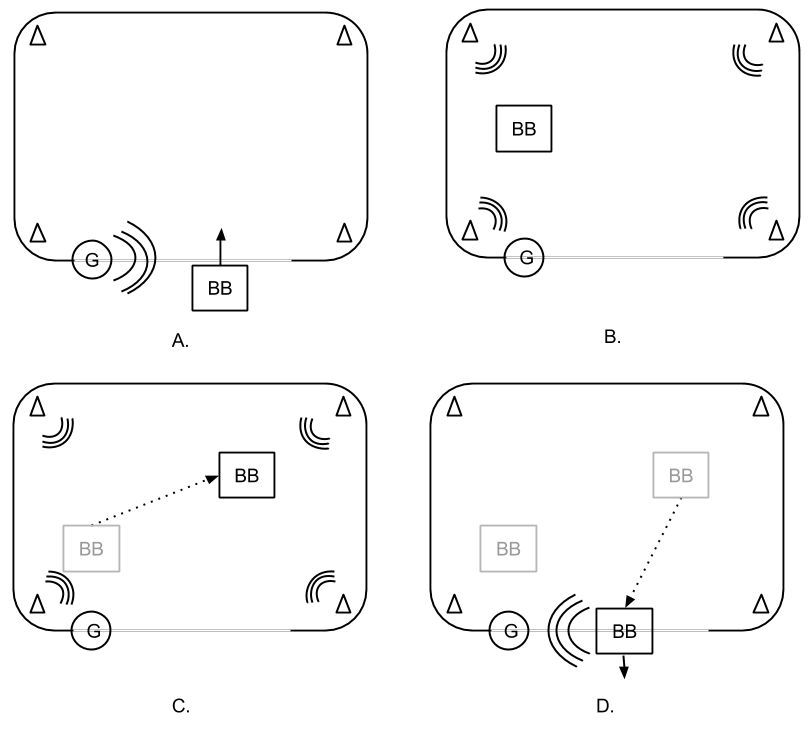
\includegraphics[width=4in,height=3in]{BumbleBeeExample.png}
		\caption{BumbleBee Architecture}
		\label{bumblebeearch}
	\end{center}
\end{figure}


\section{Implementation}
\index{Implementation@\emph{Implementation}}%


\subsection{The Gatekeeper}
\index{Gatekeeper@\emph{Gatekeeper}}%

The gatekeeper is implemented in the Python programming language so that it can remain relatively platform independent. It is comprised of three main components: the gatekeeper network service, a GUI, and a plugin interface to allow extending the systems functionality. We have implemented plugins for saving/restoring results to/from disk, graphing received signal strength from all BSSIDs across time, logging, and exporting results to a portable format for use outside BumbleBee. As part of the Honeycomb project, we also implemented a Gatekeeper plugin for uploading user tracks to the Honeycomb API. The Gatekeeper server listens on a fixed TCP port (0xb33) for requests from clients through remote procedure calls (via Python’s SimpleXMLRPCServer). Information exchange with the bumblebees is done in JSON data format. The gatekeeper administrator configures the BSSIDs addresses and minimum polling interval.


\subsection{The Bumblebee}
\index{The Bumblebee@\emph{The Bumblebee}}%

The bumblebee component is implemented as an Android application written in the Java programming language. The application performs three main tasks: automatic network detection of the Gatekeeper, negotiation with the Gatekeeper, and data collection related activities. These operations require no user interaction and thus we consider this application unobtrusive. As part of the data collection process the bumblebee application will wake up on the negotiated time interval, observe broadcasting wireless networks, and collect and store signal strength values for all requested BSSIDs. It then stamps the collected data with the offset from the time it collected the work from the Gatekeeper and returns to sleep. The periodic waking process is also used to rediscover the Gatekeeper. When the Gatekeeper is rediscovered the application once again negotiates a connection, but this time instead of accepting work it submits the collected data. The data is then discarded from the mobile device.


\subsection{Communication Mechanism}
\index{Communication Mechanism@\emph{Communication Mechanism}}%


The bumblebee mobile device communication model is shown in Figure \ref{bumblebestatediagram}. The initial state of the bumblebee is ‘Sleeping / Inactive’ (with respect to BumbleBee activities). Upon discovery of the Gatekeeper the application enters the ‘Handshake’ state. In this state the application may choose to not accept the requested task, in which case it moves back to the ‘Sleeping / Inactive’ state. If work is accepted then the application moves into the ‘Data Collection’ state. The data collection process was described in the previous section. The handshake process is described below. When the bumblebee once again discovers the Gatekeeper is once again enters the ‘Handshake’ state, but this time it transmits the collected data to the Gatekeeper. Once this is completed, the bumblebee moves back into the ‘Sleeping / Inactive’ state.

The handshake between Gatekeeper and a bumblebee client happens within the context of a single connection-oriented session and involves a simple two-way handshake. The handshake happens after the bumblebee discovers the Gatekeeper and involves either the requesting of a new data collection information or the submission of collected data. In both cases the bumblebee initially transmits its unique ID to the Gatekeeper. This provides the Gatekeeper an opportunity to perform validation of the ID (perhaps to reference a user database or possibly black/white list of IDs). Assuming the ID is validated, and the client is making a request, a response is sent listing the BSSIDs to monitor, the maximum acceptable interval between samples, and the Gatekeeper’s current timestamp. The bumblebee is now in the ‘Data Collection’ state as described above. If the client is unable to support the request it silently drops the request and transitions back to the ‘Sleeping / Inactive’ state.

If the bumblebee successfully transitioned to the ‘Data Collection’ state and the Gatekeeper is once again discovered, the handshake process again takes place. After validation the bumblebee then transmits an overall status, the original request timestamp, and the series of collected timestamped signal strength values for all BSSIDs. Regardless of the status of the request the bumblebee moves to the ‘Sleeping / Inactive’ state. The Gatekeeper will store the request, regardless of status, for later analysis. In our case, this analysis actually occurs on Honeycomb hardware.


\begin{figure}[htb] % Imported eps example.
	\begin{center}
		\ 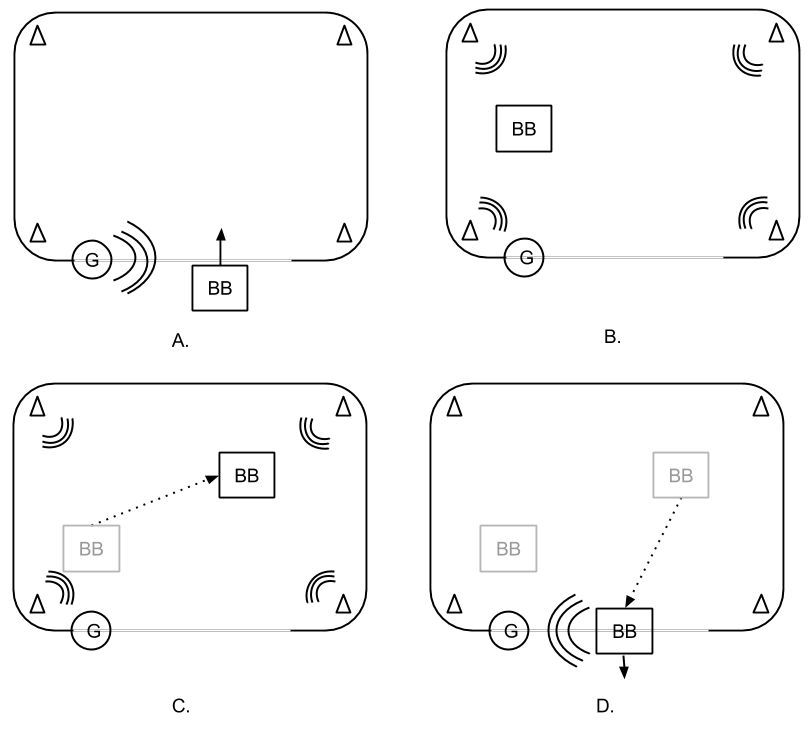
\includegraphics[width=4in,height=3in]{BumbleBeeExample.png}
		\caption{BumbleBee State Diagram}
		\label{bumblebestatediagram}
	\end{center}
\end{figure}


\chapter{Tech Overview}
\label{tech-overview}
\index{Tech Overview%
@\emph{Tech Overview}}%

In order to perform both the training phase and the estimation phase of Honeycomb's scene analysis approach to location estimation, as well as post-estimation data analysis, we implemented a mobile application as well as a web application. We employed a basic client-server architecture in which the web application acts as the server, with both the mobile application and the BumbleBee Gatekeeper as its clients. In this section, we describe the technical details of these applications.


\section{Web Application}
\index{Web Application@\emph{Web Application}}%


The most critical part of Honeycomb's implementation is the web application. It acts as the server in Honeycomb's client-server architecture, and is the place where Honeycomb performs its location estimation calculations. It also servers as the entry point into Honeycomb for site administrators to administer their sites and view user tracks. It is implemented in the Python programming language using the Django web framework \cite{django}, and is hosted on WebFaction \cite{webfaction}. It is available at https://www.honeycomb.pw \footnote{This URL will immediately prompt you to login. Please contact the author for demo credentials.}


\subsection{User Interface}
\index{User Interface@\emph{User Interface}}%


The user interface of the Honeycomb web application is intended to support location administrators, and is designed using the Bootstrap CSS and Javascript framework \cite{bootstrap}. Once logged in to the application, location administrators can view the locations that they administer, as well as create new locations within the app. By allowing a single person to administer multiple locations in this manner, we support an administrator's ability to own the location estimation deployment at multiple sites. Locations created through this interface will be exposed via the API (described in more detail later) for use in the location estimation phases. Site administrators can also view the currently active as well as past fingerprint sessions, including the raw signal strength measurements for each fingerprint in the session. Additionally, individual user tracks can be viewed, including both the raw signal strength measurements of the track as well as a table showing each timestamp offset and the estimated location of the user at that time. 
	

\subsection{REST API}
\index{REST API@\emph{REST API}}%


Honeycomb's API is its programmatic interface with the clients in the client-server architecture. It is built using Representational State Transfer (REST) principles \cite{fielding2002principled}, and the JSON data format \cite{json}, both of which are standard for programmatic interfaces today. It exposes four endpoints in order to facilitate location estimate, which are described below.


\paragraph{Tokens}
\index{Tokens@\emph{Tokens}}%

The Honeycomb API authentication mechanism is token based. The token endpoint accepts a set of credentials and returns a token, which can be used to interact with the rest of the API. This is the only endpoint that accepts credentials, all others use the provided token for authentication. The benefit of this authentication mechanism is that the site administrator must only input their credentials once, and the client application does not need to store those credentials. This provides the administrator with a measure of security, as their credentials cannot be stolen if they are not stored. Should the client experience a breach of security of the given token, that token can be revoked on the server without the administrator's intervention, and does not require them to change their password. 


\paragraph{Locations}
\index{Locations@\emph{Locations}}%

The location endpoint provides a list of locations administered by the owner of the provided authentication token. Honeycomb allows a single administrator to administer multiple locations, and exposing those locations in this endpoint allows clients to present the administrator with a selection of locations that they administer when relevant. This means that a single administrator can use the same Honeycomb mobile application, and even the same BumbleBee Gatekeeper application, at multiple sites, while still maintaining the integrity of the data gathered at each site. 


\paragraph{Fingerprint Sessions}
\index{Fingerprint Sessions@\emph{Fingerprint Sessions}}%

The fingerprint session endpoint provides clients with an interface through which to upload a full fingerprint session, including multiple signal strength measurements for each fingerprint at the given location. In order to successfully create a new fingerprint session, the provided authentication token must represent the administrator of the provided site. 

The fingerprint session endpoint does not support updating of a single fingerprint's signal strength measurements. Instead, fingerprints uploaded to this endpoint are considered to be the full set of fingerprints for a session. This decision was made because any change to a given fingerprint's measurements likely propagated to other fingerprints as well. For instance, if a new display was set up somewhere in the store, it likely changed the distribution of signal strengths throughout the space. Therefore, if the site administrator wants to add a fingerprint at the new display, they must re-fingerprint the entire space. Every session uploaded through this endpoint is considered to be the latest fingerprint session for the given site, and is therefore marked as the active session, and all other session are marked as inactive. Thus, all user tracks uploaded are compared against the most recent fingerprint session uploaded.


\paragraph{User Tracks}
\index{User Tracks@\emph{User Tracks}}%

The user track endpoint provides clients with an interface through which to upload user tracks, including timestamped signal strength measurements and any identifying information about the user that the client wishes to provide. In order to successfully create a user track, the provided authentication token must represent the administrator of the provided site. Although BumbleBee is used in this paper as the user track client, Honeycomb will accept data from any source, provided that the client provides the appropriate authentication token. Tracks uploaded in this way are stored in the database and queued for asynchronous processing, as described below.

		
\subsection{Asynchronous Processing}
\index{Asynchronous Processing@\emph{Asynchronous Processing}}%


Honeycomb's algorithms involve some measure of complex processing. In order to prevent this complex processing from causing a bottleneck in the HTTP request/response cycle during API requests, and thus to ensure scalability of the application, Honeycomb employs a system of asynchronous processes. These asynchronous processes use Celery \cite{celery} as an asynchronous task manager and Redis \cite{redis} as a message queue. Thus, the Honeycomb API accepts raw data through its endpoints, stores it in a PostgreSQL \cite{postgresql} database, adds a message to Redis, and returns a response to the client immediately. At some point after the response is returned (usually almost immediately, but potentially some larger amount of time), Celery dequeues the message from Redis and invokes the appropriate asynchronous task. The task processes the raw data and stores the resulting data in the database. The two main asynchronous tasks are described below.


\paragraph{Asynchronous Fingerprint Processing}


Honeycomb's API supports the uploading of fingerprints with multiple signal strength measurements for each Wi-Fi access point. The purpose for this is to gather multiple signal strength measurements over time in order to avoid abnormally large or small instantaneous values. This raw data is stored as-is, by the API endpoint. The asynchronous process then calculates the mean of the measurements \cite{turner2011empirical} and stores those in the database as well. It is against these processed values that the user tracks are compared.


\paragraph{Asynchronous User Track Processing}


When Honeycomb's API receives a user track, it stores the data as-is in the database. The asynchronous task then performs the Euclidean distance algorithm (see section \ref{honeycombapproach}) against the user track and the currently active fingerprint, and stores the result in the database. When a site administrator views a user track, this calculation has already been performed, and can thus be rendered efficiently.
	

\section{Mobile Application}
\index{Mobile Application@\emph{Mobile Application}}%

Honeycomb's training phase is implemented as an Android application in the Java programming language. Upon first opening the application, the site administrator is prompted to log in with their Honeycomb credentials. The mobile application then makes use of the Honeycomb token API endpoint, and exchanges the supplied credentials for a token, which is cached locally. It then immediately queries the location endpoint and presents the administrator with a list of administered locations so that they can choose which location they are about to fingerprint. 

Once the administrator is logged in and a location is chosen, they are presented with a form in which to input a list of BSSIDs of Wi-Fi access points to poll for during each fingerprint and a length of time to poll. Then, the administrator must physically locate themselves at each of the desired polling points. For each point, the administrator is prompted to input a description of the point for later identification. The mobile app then performs the requested polling, and the administrator can move on to the next point. Once a fingerprint session is complete, the application uploads the full session to the fingerprint session API endpoint, along with the administrator authentication token and the site identifier provided by the location endpoint. At this point, the training phase is complete. At any point in the future, the administrator can perform the entire process again in order to create an updated fingerprint session.


\section{BumbleBee plugin}
\index{BumbleBee plugin@\emph{BumbleBee plugin}}%


As stated earlier, in order to prove Honeycomb's viability as a location estimation product, we employed BumbleBee as a user track gathering mechanism. We leveraged BumbleBee's plugin architecture, and wrote a Honeycomb specific plugin for uploading user tracks. Like the Honeycomb mobile app, this plugin prompts the administrator for their Honeycomb credentials and exchanges these credentials for a token. It then uses this token to gather the administrator's locations and prompts them to select the location for which they are gathering user tracks. It then uploads user tracks in bulk to the Honeycomb API, where Honeycomb can then process the data.

\chapter{Testing and Results}
\label{results}
\index{Testing and Results%
	@\emph{Testing and Results}}%

In order to test the effectiveness of Honeycomb as an indoor location estimation tool, we ran a series of test variants in a single location and mapped out the results for comparison. In this section we present the testing setup and the results. 


\section{Testing Setup}
\index{Testing Setup@\emph{Testing Setup}}%

 A map of our location can be seen in Figure \ref{loc1_path}. This space is roughly 24 feet wide by 42 feet long for a total of approximately 1000 square feet. The dotted line in the figure represents our actual route through the space, which we repeated for each test variant. The shaded areas and dark lines are walls or other inaccessible areas in the actual location, although they could just as easily represent shelving or other displays in the grocery store scenario. The solid black dots are our fingerprint locations.
 
 We employed six Wi-Fi access points of various makes and models for our testing \footnote{Linksys WRT54GL, Linksys WRT600N, Linksys WRT54G2, Netgear WNR2000, and two Netgear WGR614s}. We chose these access points because they are popular brands which can be found in wide use today, and thus represent a real world scenario. Our mobile device, both for fingerprinting and user track collection was a Samsung Galaxy S5. 
 
 Unlike much of the location estimation research in this area, we did not make a regularly spaced grid of fingerprints, choosing instead to place fingerprints only at notable locations in the space. This does decrease precision slightly, but also makes the fingerprinting process less painful, which is an important factor in adoption in a real world deployment. However, even with fingerprints only at notable locations, a sufficient density of fingerprints will still provide an adequate level of precision for our intended scenarios. In our tests, we placed 10 fingerprints in a 1000 square foot space, which is roughly one fingerprint for every 10 square feet. In the scenarios that we described in chapter \ref{introduction}, we believe that would be adequate precision. 


\begin{figure}[htb] % Imported eps example.
	\centering
	\ 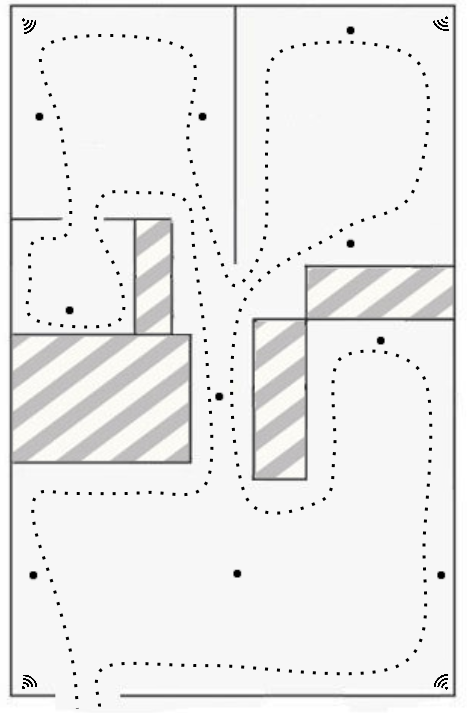
\includegraphics[width=2.8in,height=4in]{loc1_path.png}
	\caption{Map of location, with fingerprint points and walking path}
	\label{loc1_path}
\end{figure}

\section{Test Variants}
\index{Test Variants@\emph{Test Variants}}%


While there are many possible variables that could be tested, from Wi-Fi access point signal reliability to individual mobile phone capabilities, the two main variables that are most relevant to viability of Honeycomb are the number of access points in the space and the length of the poll time for each fingerprint.

The importance of the number of access points in the space is obvious. We make an assumption in our tests that a single access point, or even two or three access points, is simply not enough to get a reliable estimation. Therefore, we introduced two major test variants, one with four access points and one with six. 

The less obvious, but potentially more crucial variable is the length of time spent polling each fingerprint location. As described in chapter \ref{tech-overview}, Honeycomb is capable of taking multiple signal strength measurements for each fingerprint location so as to avoid incorrect measurements due to abnormally large or small instantaneous values. The question, then, is what amount of time spent polling a single fingerprint is enough to get an accurate measurement. Therefore, we introduced three test variants for polling time: 10 seconds, 20 seconds, and 30 seconds.

Thus, with these two variables and their variants, we have six independent tests: four and six access points, each with polling times of 10, 20, and 30 seconds. For the four access point tests, we placed an access point at each of the four corners of the space, and for the six access point tests, we placed two additional access points at the mid point of the longer walls on either side. For each test we independently fingerprinted the entire space, and then walked the route mapped out in Figure \ref{loc1_path}.


\section{Results}
\index{Results@\emph{Results}}%


Figures \ref{loc1_4ap_10s}, \ref{loc1_6ap_10s}, \ref{loc1_4ap_20s}, \ref{loc1_6ap_20s}, \ref{loc1_4ap_30s}, and \ref{loc1_6ap_30s} represent the results of each of our test variants. In these maps, we have placed a large red dot at the fingerprint which represents the first estimation of the user's location. From there, we have placed numbered red lines to each of the subsequent fingerprint locations estimated to be the user's location. It is important to note that these lines are not intended to represent the user's actual movement through the space, but are simply handy references for showing general movement from one fingerprint area to another. As such, these lines are free to move through walls, and can be either straight or curved, depending on need.  It is also important to note that the number of lines in each map can vary significantly, due to the fact that the same fingerprint location can be considered the user's location at multiple successive timestamps, and we have only represented instances of location change in these result maps. 


\begin{figure}
	\centering
	\begin{minipage}{0.45\textwidth}
		\ 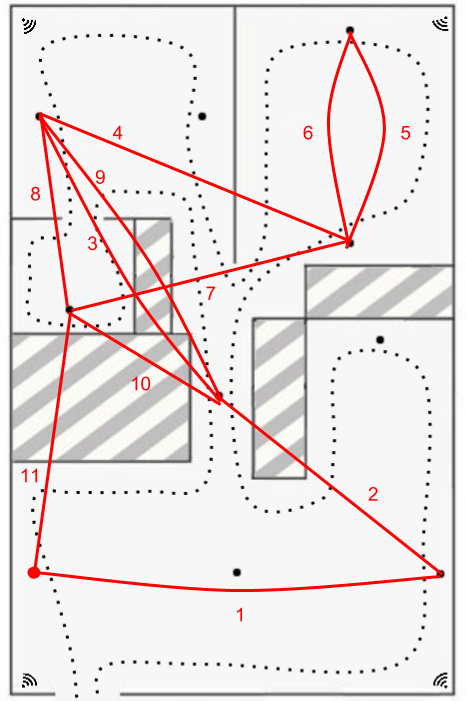
\includegraphics[width=2in,height=2.8in]{loc1_4ap_10s.png}
		\caption{Results with four access points and a ten second polling time}
		\label{loc1_4ap_10s}
	\end{minipage}\hfill
	\begin{minipage}{0.45\textwidth}
		\centering
		\ 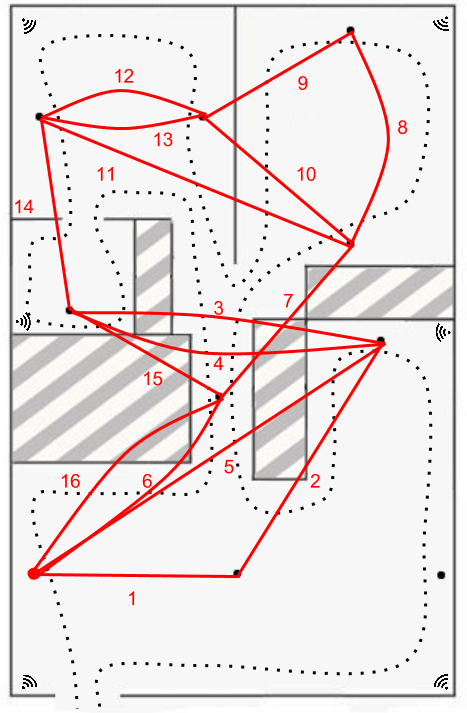
\includegraphics[width=2in,height=2.8in]{loc1_6ap_10s.png}
		\caption{Results with six access points and a ten second polling time}
		\label{loc1_6ap_10s}
	\end{minipage}
\end{figure}

\begin{figure}
	\centering
	\begin{minipage}{0.45\textwidth}
		\ 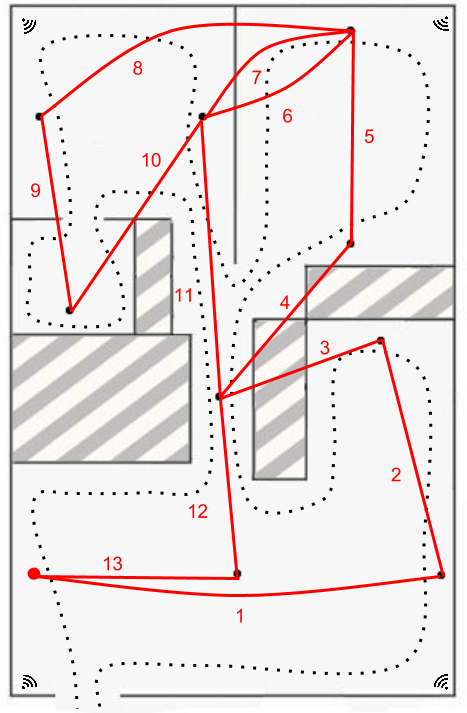
\includegraphics[width=2in,height=2.8in]{loc1_4ap_20s.png}
		\caption{Results with four access points and a twenty second polling time}
		\label{loc1_4ap_20s}
	\end{minipage}\hfill
	\begin{minipage}{0.45\textwidth}
		\centering
		\ 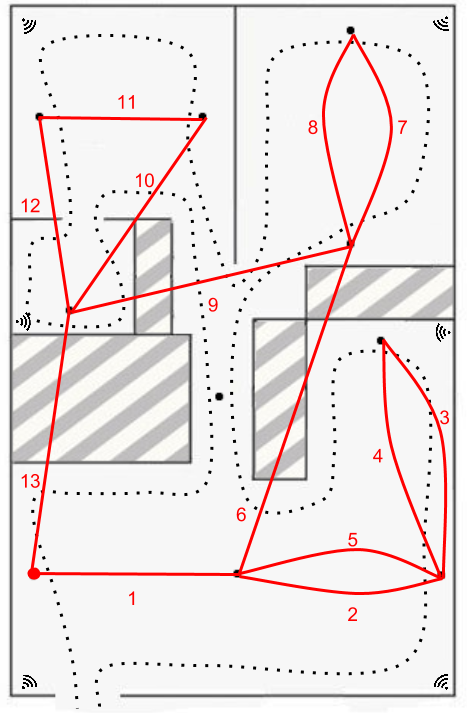
\includegraphics[width=2in,height=2.8in]{loc1_6ap_20s.png}
		\caption{Results with six access points and a twenty second polling time}
		\label{loc1_6ap_20s}
	\end{minipage}
\end{figure}

\begin{figure}
	\centering
	\begin{minipage}{0.45\textwidth}
		\ 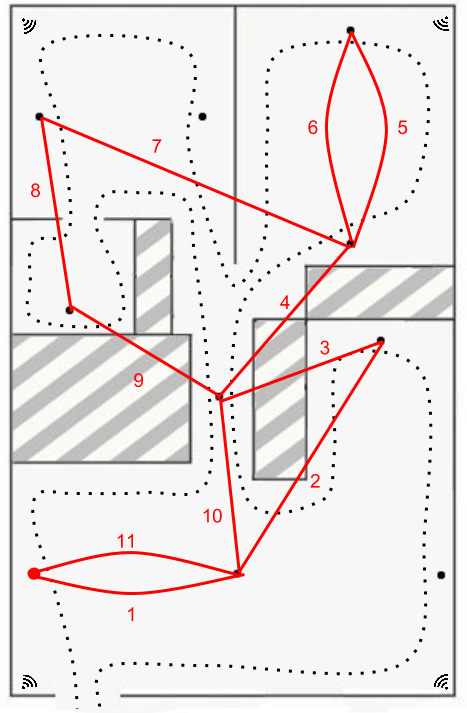
\includegraphics[width=2in,height=2.8in]{loc1_4ap_30s.png}
		\caption{Results with four access points and a thirty second polling time}
		\label{loc1_4ap_30s}
	\end{minipage}\hfill
	\begin{minipage}{0.45\textwidth}
		\centering
		\ 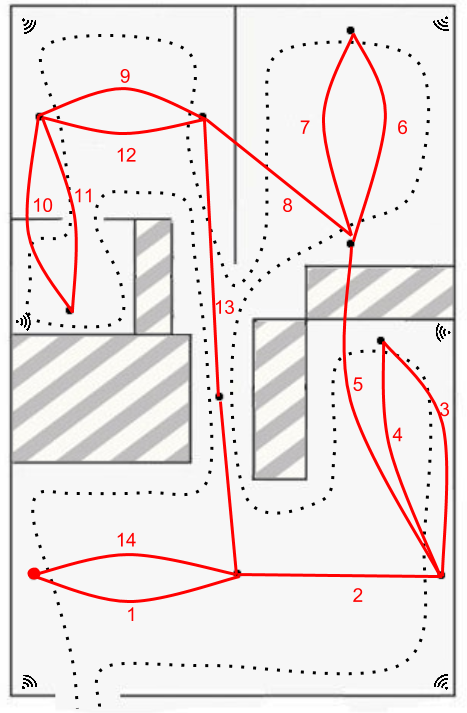
\includegraphics[width=2in,height=2.8in]{loc1_6ap_30s.png}
		\caption{Results with six access points and a thirty second polling time}
		\label{loc1_6ap_30s}
	\end{minipage}
\end{figure}


Figures \ref{loc1_4ap_10s} and \ref{loc1_6ap_10s} represent the two test variants with 10 second polling times. These variants are clearly quite susceptible to getting lost, particularly in the upper left quadrant of the map. Interestingly, both variants do seem to recover from their failure points, particularly in the upper right quadrant of the map. However, regardless of their recovery ability, both of these variants have significant issues with actual user locations and are not particularly useful as location estimators. 


Figures \ref{loc1_4ap_20s} and \ref{loc1_6ap_20s} represent the 20 second polling time variants. These are quite clearly far more accurate than the 10 second polling time variants. In Figure \ref{loc1_4ap_20s}, Honeycomb had a bit of trouble toward the upper middle section of the map at lines 6 and 7, but quickly recovered for the duration. Similarly, Figure \ref{loc1_6ap_20s} has an extra stopover at a fingerprint, represented by line 9, but also quickly recovered. It also has an aberration in which in line 13 goes straight to the end point, skipping a fingerprint in the middle of the map.

Figure \ref{loc1_4ap_30s} and \ref{loc1_6ap_30s} represent the 30 second polling time variants. Like the 20 second variants, both of these maps skip fingerprints a couple of times, but quickly recover and generally follow the correct movement trend. 

\chapter{Conclusions and Future Work}
\label{discussion}
\index{Conclusions and Future Work%
	@\emph{Conclusions and Future Work}}%


While our results do not show perfect location tracking of a user, we believe that they do make it clear that Honeycomb is a viable product for indoor location estimation, provided an adequate number of access points and fingerprint polling time. However, in performing our tests we discovered that fingerprinting itself can be a painful process, particularly with longer poll times. One way to alleviate this pain is to decrease fingerprint density in such a way that supports only the minimum viable precision necessary at a given location. Thus, fingerprint density becomes a knob that one can turn to fine tune an individual deployment of Honeycomb, and must be decided on a case by case basis. 

While this paper has proven Honeycomb's effectiveness as a product, there are still many things that must be done in order to make Honeycomb market ready. Most importantly, the user interfaces need significant work, particularly the web interface for viewing a user track, which is currently a table of timestamps and fingerprints. The result maps in this paper were created manually, but a programmatic rendering of these maps in the web interface would be preferable. 

Additionally, the web interface currently only has the ability to view each user track individually. In order to make this information useful, an aggregating and reporting function is needed which can provide information about trends in user tracks rather than data about any specific track. With this information, a site administrator could more effectively manage their space in order to maximize visibility and flow. 

However, despite shortcomings in user interfaces, we believe that Honeycomb's current incarnation represents the backbone of a viable location estimation product, and that with only relatively minor adjustments could potentially be employed in real world scenarios. 


%%%%%%%%%%%%%%%%%%%%%%%%%%%%%%%%%%%%%%%%%%%%%%%%%%%%%%%%%%%%%%%%%%%%%%
% Appendix/Appendices                                                %
%%%%%%%%%%%%%%%%%%%%%%%%%%%%%%%%%%%%%%%%%%%%%%%%%%%%%%%%%%%%%%%%%%%%%%
%
% If you have only one appendix, use the command \appendix instead
% of \appendices.
%
%\appendices
%\index{Appendices@\emph{Appendices}}%

%\chapter{Lerma's Appendix}
\index{Appendix!Lerma's Appendix@\emph{Lerma's Appendix}}%
The source \LaTeX{} file for this document is no longer quoted in
its entirety in the output document. A \LaTeX{} file can 
include its own source by using the command
\cn{verbatiminput\{\cn{jobname}\}}.



%%%%%%%%%%%%%%%%%%%%%%%%%%%%%%%%%%%%%%%%%%%
\chapter{My Appendix \#2}
\index{Appendix!My Appendix \#2@\emph{My Appendix \#2}}%
\section{The First Section}
This is the first section.
This is the second appendix.

\section{The Second Section}
This is the second section of the second appendix.

\subsection{The First Subsection of the Second Section}
This is the first subsection of the second section of the second appendix.

\subsection{The Second Subsection of the Second Section}
This is the second subsection of the second section of the second appendix.

\subsubsection{The First Subsubsection of the Second Subsection of
		the Second Section}
This is the first subsubsection of the second subsection of the
second section of the second appendix.

\subsubsection{The Second Subsubsection of the Second Subsection
		of the Second Section}
This is the second subsubsection of the second subsection of the
second section of the second appendix.


%%%%%%%%%%%%%%%%%%%%%%%%%%%%%%%%%%%%%%%%%%%
\chapter{My Appendix \#3}
\index{Appendix!My Appendix \#3@\emph{My Appendix \#3}}%

\section{The First Section}
This is the first section.
This is the third appendix.

\section{The Second Section}
This is the second section of the third appendix.





%%%%%%%%%%%%%%%%%%%%%%%%%%%%
% Generate the index.						     %
%%%%%%%%%%%%%%%%%%%%%%%%%%%%%%%%%%%%%%%%%%%%%%%%%%%%%%%%%%%%%%%%%%%%%%
%								     %
% NOTE: For master's theses and reports, NOTHING is permitted to     %
%	come between the bibliography and the vita. This section     %
%	to generate the index (if used) MUST be moved to before      %
%	the bibliography section.				     %
%								     %
%\printindex%    % Include the index here. Comment out this line      %
%		% with a percent sign if you do not want an index.   %
%%%%%%%%%%%%%%%%%%%%%%%%%%%%%%%%%%%%%%%%%%%%%%%%%%%%%%%%%%%%%%%%%%%%%%


%%%%%%%%%%%%%%%%%%%%%%%%%%%%%%%%%%%%%%%%%%%%%%%%%%%%%%%%%%%%%%%%%%%%%%
% Generate the bibliography.					     %
%%%%%%%%%%%%%%%%%%%%%%%%%%%%%%%%%%%%%%%%%%%%%%%%%%%%%%%%%%%%%%%%%%%%%%
%								     %
% NOTE: For master's theses and reports, NOTHING is permitted to     %
%	come between the bibliography and the vita. The command      %
%	to generate the index (if used) MUST be moved to before      %
%	this section.						     %
%								     %
\nocite{*}      % This command causes all items in the 		     %
                % bibliographic database to be added to 	     %
                % the bibliography, even if they are not 	     %
                % explicitly cited in the text. 		     %
		%						     %
\bibliographystyle{plain}  % Here the bibliography 		     %
\bibliography{diss}        % is inserted.			     %
\index{Bibliography@\emph{Bibliography}}%			     %
%%%%%%%%%%%%%%%%%%%%%%%%%%%%%%%%%%%%%%%%%%%%%%%%%%%%%%%%%%%%%%%%%%%%%%


%%%%%%%%%%%%%%%%%%%%%%%%%%%%%%%%%%%%%%%%%%


%%%%%%%%%%%%%%%%%%%%%%%%%%%%%%%%%%%%%%%%%%%%%%%%%%%%%%%%%%%%%%%%%%%%%%
% Vita page.							     %
%%%%%%%%%%%%%%%%%%%%%%%%%%%%%%%%%%%%%%%%%%%%%%%%%%%%%%%%%%%%%%%%%%%%%%

\begin{vita}
TODO: VITA

\end{vita}

\end{document}
